%!TEX root = presentation.tex

\section{Approche orientée événements}

\begin{frame}
	\begin{minipage}{0.5\columnwidth}
		
		\tableofcontents[
		currentsubsection,
		sectionstyle=show/shaded,
		subsectionstyle=show/show/hide,
		]
	\end{minipage}\hfill
	\begin{minipage}{0.5\columnwidth}
		\inputTikZ{0.7}{img/tikz/approche2.tex}
	\end{minipage}
\end{frame}


\subsection{Modèle événementiel}


%\begin{frame}{Domain Driven Design}
%\begin{block}{DDD - Modélisation pilotée par le domaine \cite{Evans2003}}
%	Définir un langage et une vision partagée 
%	par tous les acteurs de l'application pour construire l'application.
%\end{block}
%	Agrégat : groupe d'objets associés considérés comme un tout vis-à-vis des 
%	modifications de données (Scène, Maillage, Géométrie)
%	
%	Agrégat racine: Seul objet accessible de l'extérieur (Scène, User) -> assurer 
%	l'intégrité du contenu à l'intérieur de l'agrégat.
%	
%	-> Proposer un langage partagé et des 
%	événements pour la manipulation et la visualisation 3D
%\end{frame}
%
%\begin{frame}{Contribution : Description des événements 3D}
%
%\begin{table}
%	\centering
%	\small
%	\caption{Exemple d'événements de 
%		l'agrégat Maillage}
%	\label{tab:extraitevent}
%	\begin{tabular}{lll}
%		\textbf{Événement}& \textbf{Dénomination} & \textbf{Description} \\ \hline
%		%\textbf{Agrégat Maillage}  &                      &             \\ \hline
%		Maillage ajouté (*)&     meshAdded                 
%		&  \begin{tabular}[c]{@{}l@{}} Un maillage a été ajouté dans\\  la Scène à 
%			partir d'une géométrie\\ de la 
%			bibliothèque \end{tabular}  \\\hline
%		Maillage déposé (*) &     meshDropped               
%		&      \begin{tabular}[c]{@{}l@{}} Un maillage a été déposé dans 
%			\\l'env. 3D de la Scène à 
%			partir \\d'une géométrie de la bibliothèque \end{tabular} \\\hline
%		Maillage supprimé & meshRemoved       &        
%		\begin{tabular}[c]{@{}l@{}} 
%			Un maillage a été 
%			supprimé \\de la Scène \end{tabular}      \\\hline
%		Maillage translaté &   meshTranslated  	 &    \begin{tabular}[c]{@{}l@{}} 
%			Un 
%			maillage a 
%			subi une translation \\dans la Scène \end{tabular}          
%	\end{tabular}
%\end{table}
%\end{frame}
%
%\begin{frame}{Event Sourcing}
%\begin{block}{ES \cite{Fowler2005EventSourcing}}
%	Enregistrer 
%	chaque modification de l'état de l'application sous la forme d'un 
%	événement.
%\end{block}
%Événement : s'applique à un agrégat, possède un type et des paramètres.
%
%Exemple: $AggScene1::meshAdded(''cube1'',geometry1)$
%
%-> Journal d'événements = source unique de vérité dans 
%l'application
%\end{frame}
%
%\begin{frame}{Command Query Responsability Segregation}
%\begin{block}{CQRS \cite{Young2009}}
%	Séparer : 
%	\begin{itemize}
%		\item la partie commande (écriture) : validation des règles métiers
%		\item de la partie requête (lecture) dans une application : passage à 
%		l'échelle, cohérence éventuelle.
%	\end{itemize}
%\end{block}
%
%La collaboration implique une forte demande partie écriture (SEC) et partie
%lecture (visualisation collaborative à synchronicité variable)
%
%
%-> Valider toute donnée entrante (utilisateur ou réseau) selon les 
%règles métiers définies. 
%
%-> Flexibilité de la visualisation du contenu généré
%avec les projections.
%\end{frame}
\begin{frame}{Patron de conception adaptés}
\only<1->{
	\begin{textblock*}{65mm}(0.05\textwidth,0.2\textheight)
		\begin{exampleblock}{DDD \cite{Vernon2013}}
			\begin{itemize}
				\item Langage partagé
				\item Contexte
				\item Règles métier
			\end{itemize}
		\end{exampleblock}
	\end{textblock*}
	
	\begin{textblock*}{65mm}(0.4\textwidth,0.2\textheight)
		\begin{exampleblock}{ES \cite{Fowler2003}}
			\begin{itemize}
				\item Un changement = un événement
				\item Événements immuables
				\item Support de l'historique
			\end{itemize}
		\end{exampleblock}
	\end{textblock*}
	
	\begin{textblock*}{65mm}(0.8\textwidth,0.2\textheight)
		
		\begin{exampleblock}{CQRS \cite{Young2010}}
			\begin{itemize}
				\item Séparer écriture / lecture
				\item Validation des données 
				\item Cohérence éventuelle 
			\end{itemize}
		\end{exampleblock}
		
	\end{textblock*}
}
\only<2>{
	\begin{textblock*}{15cm}(0.05\textwidth,0.55\textheight)
		
		\begin{exampleblock}{Définition des événements}
			
			Création du langage partagé à partir des observations des précédentes 
			expérimentations.\\
			Définition du contexte pour tous les objets liés à l'application.\\
			Définitions des événements associés à ces objets.
		\end{exampleblock}
		
	\end{textblock*}
	
	\begin{textblock*}{15cm}(0.05\textwidth,0.82\textheight)
		
		\begin{exampleblock}{CQRS+ES}
			
			Favoriser l'autonomie de l'utilisateur.\\
			Proposer différentes vues des mêmes données (3D, monitoring, 
			historique)\\
			Approche faiblement couplée adaptée à la collaboration (forte demandes 
			en 
			écriture et en lecture)
		\end{exampleblock}
		
	\end{textblock*}
}
\end{frame}

\begin{frame}{Modèle général \cite{Desprat2016}}
\centering
		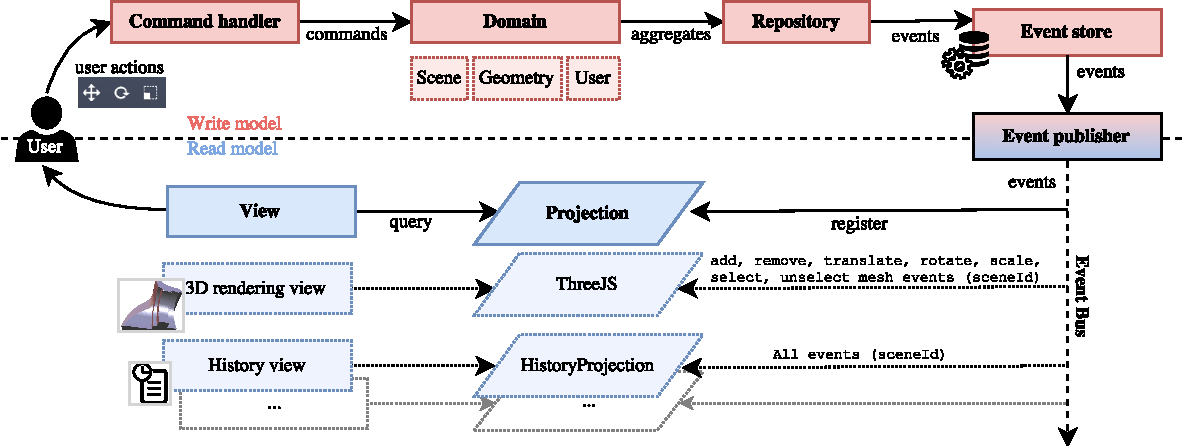
\includegraphics[width=0.9\columnwidth]{eps/cqrs3.pdf}

\end{frame}


\begin{frame}{Modèle général : exemple (translation d'un cube par User A)}

	\begin{figure}
		\centering
		\includegraphics[width=0.5\columnwidth]{eps/example10.eps}
	
	\end{figure}

\textit{Publié dans }
\end{frame}



\begin{frame}{Architecture réseau hybride orientée \cite{Desprat2017}
événements}
	{\centering
	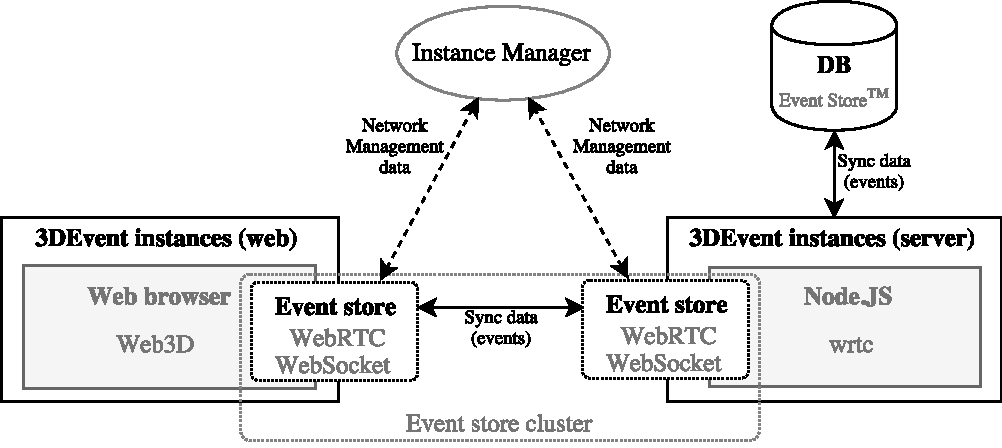
\includegraphics[width=0.7\columnwidth]{eps/archi.pdf}}


\begin{itemize}
	\item Améliorer le passage à l'échelle en intégrant le modèle événementiel
	\item Réduire les contraintes de collaboration : concurrence optimiste, réseau 
	moins dense
\end{itemize}

\end{frame}

\subsection{Prototype 3DEvent}

\begin{frame}{3DEvent - Prototype de l'éditeur collaboratif 3D}
	\begin{minipage}{.5\columnwidth}
	Fonctionnalités
	\begin{itemize}
		\item Transformations haut niveau (t,r,h)
		\item Visualisation, navigation
		\item Import de modèles 3D
	\end{itemize}
	Intégration CQRS+ES
	\begin{itemize}
		\item Interface orientée tâche 
		\item Sélection fantôme
	\end{itemize}
	\end{minipage}\hfill
	\begin{minipage}{.5\columnwidth}
		\begin{figure}
			\centering
			\includegraphics[width=\columnwidth]{eps/1translatehisto.eps}
			\caption{Translation // historique}
		\end{figure}
	\end{minipage}
\end{frame}



\begin{frame}{Expérimentation approche orientée événements}
		\begin{columns}[onlytextwidth]
		\column{0.48\textwidth}
		\begin{alertblock}{Objectif}
			Intégration du modèle événementiel possible\\
			Efficacité dans la réalisation collaborative\\
			Possibilité d'analyse des données
		\end{alertblock}
		\column{0.5\textwidth}
		
		\begin{block}{Description}
			Assemblage collaboratif de modèles 3D ou création de scène libre.\\
			Internet (hétérogène) \\
			Prototype 3DEvent.\\
		\end{block}
	\end{columns}

	\begin{columns}[onlytextwidth]
		\column{0.48\textwidth}
			\begin{block}{Critères d'évaluation}
				\begin{itemize}
					\item Qualité de la collaboration : cohérence, fiabilité, réactivité
					\item Efficience : temps et sentiment d'efficacité
				\end{itemize}
			\end{block}
		\column{0.55\textwidth}
			\scriptsize
			\begin{table}[ht]
			\centering
			\caption{Modèles}
			\begin{tabular}{cccc}
				\textbf{Modèle}  & \textbf{Nb parties} &  \textbf{Triangles} & 
				\textbf{Taille 
				tot.}  \\ \hline
				Rotor      &   10  &    62k & 4Mo \\
				Camera box        &   12  &    67k & 5Mo        \\
				Car      &   16  &      170k & 8Mo \\ 
				Living room      &   16  &      200k & 9Mo \\\hline
			\end{tabular}
		\end{table}
	\end{columns}
\end{frame}

\subsection{Résultats et discussion}
\begin{frame}{Résultats des questionnaires}

	\centering
	\includegraphics[width=\columnwidth]{eps/questionnaire.eps}


\end{frame}

\begin{frame}{Analyse des données}

	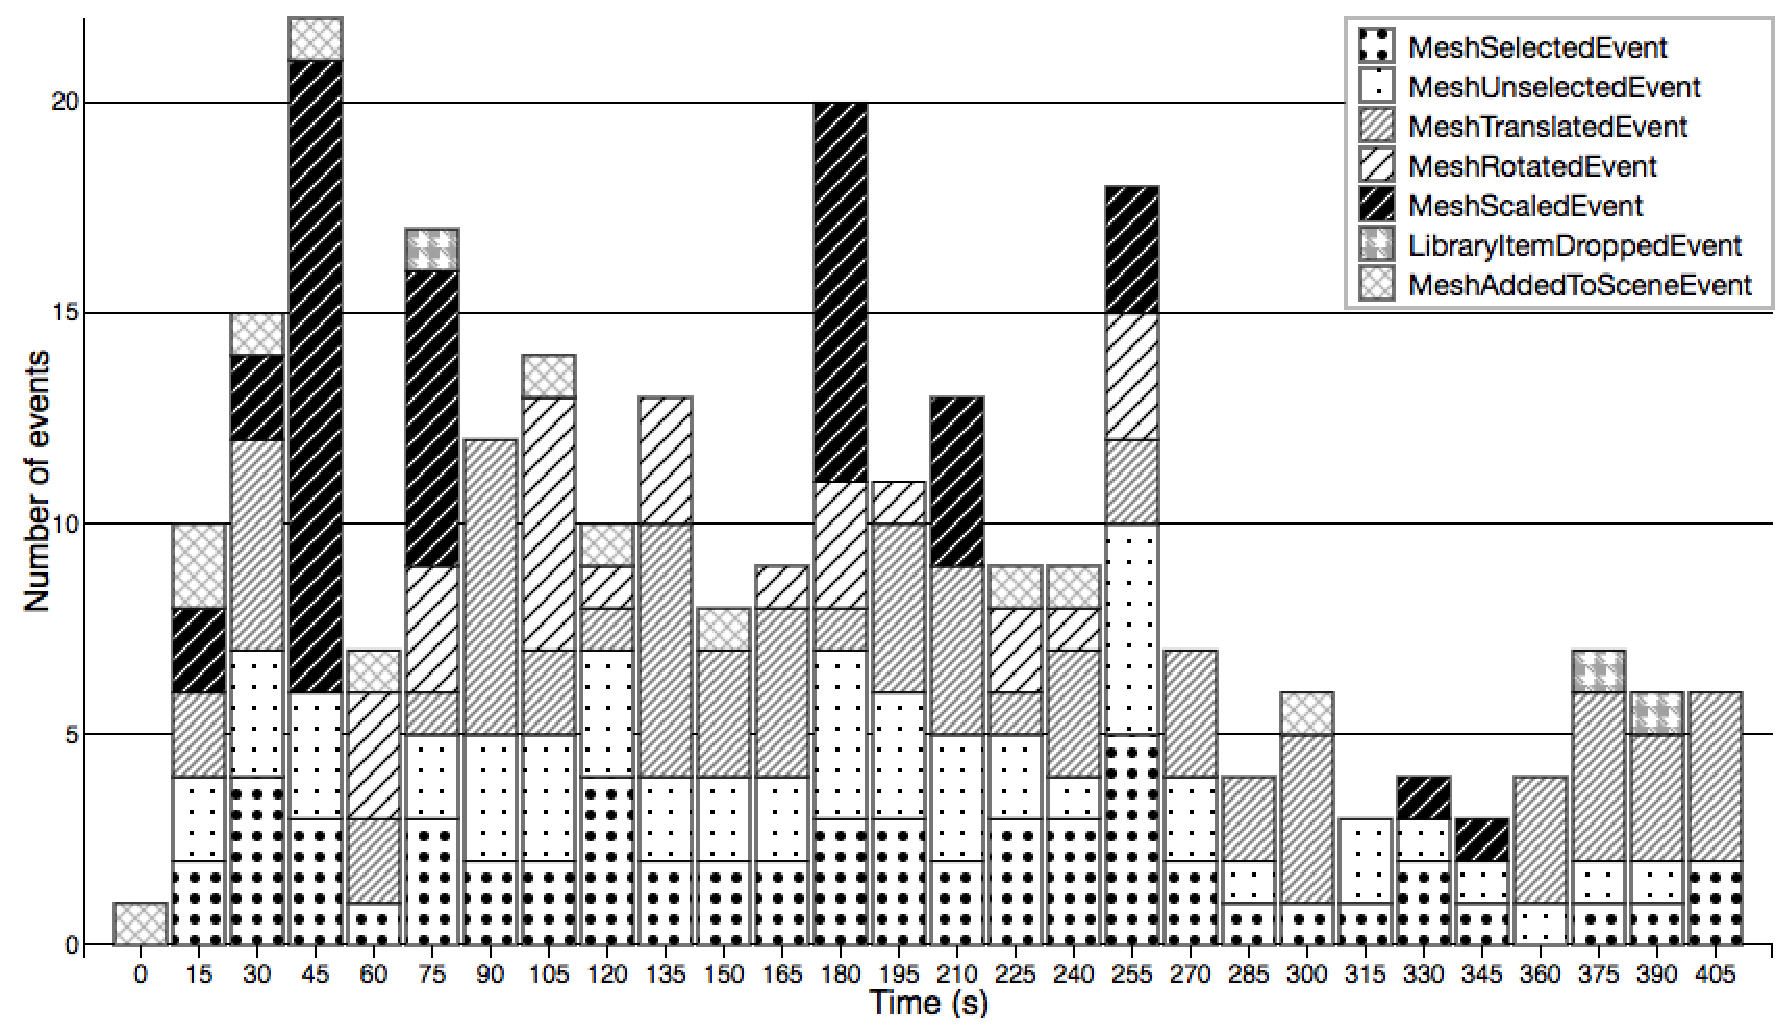
\includegraphics[width=0.8\textheight]{eps/byevents.eps}\\
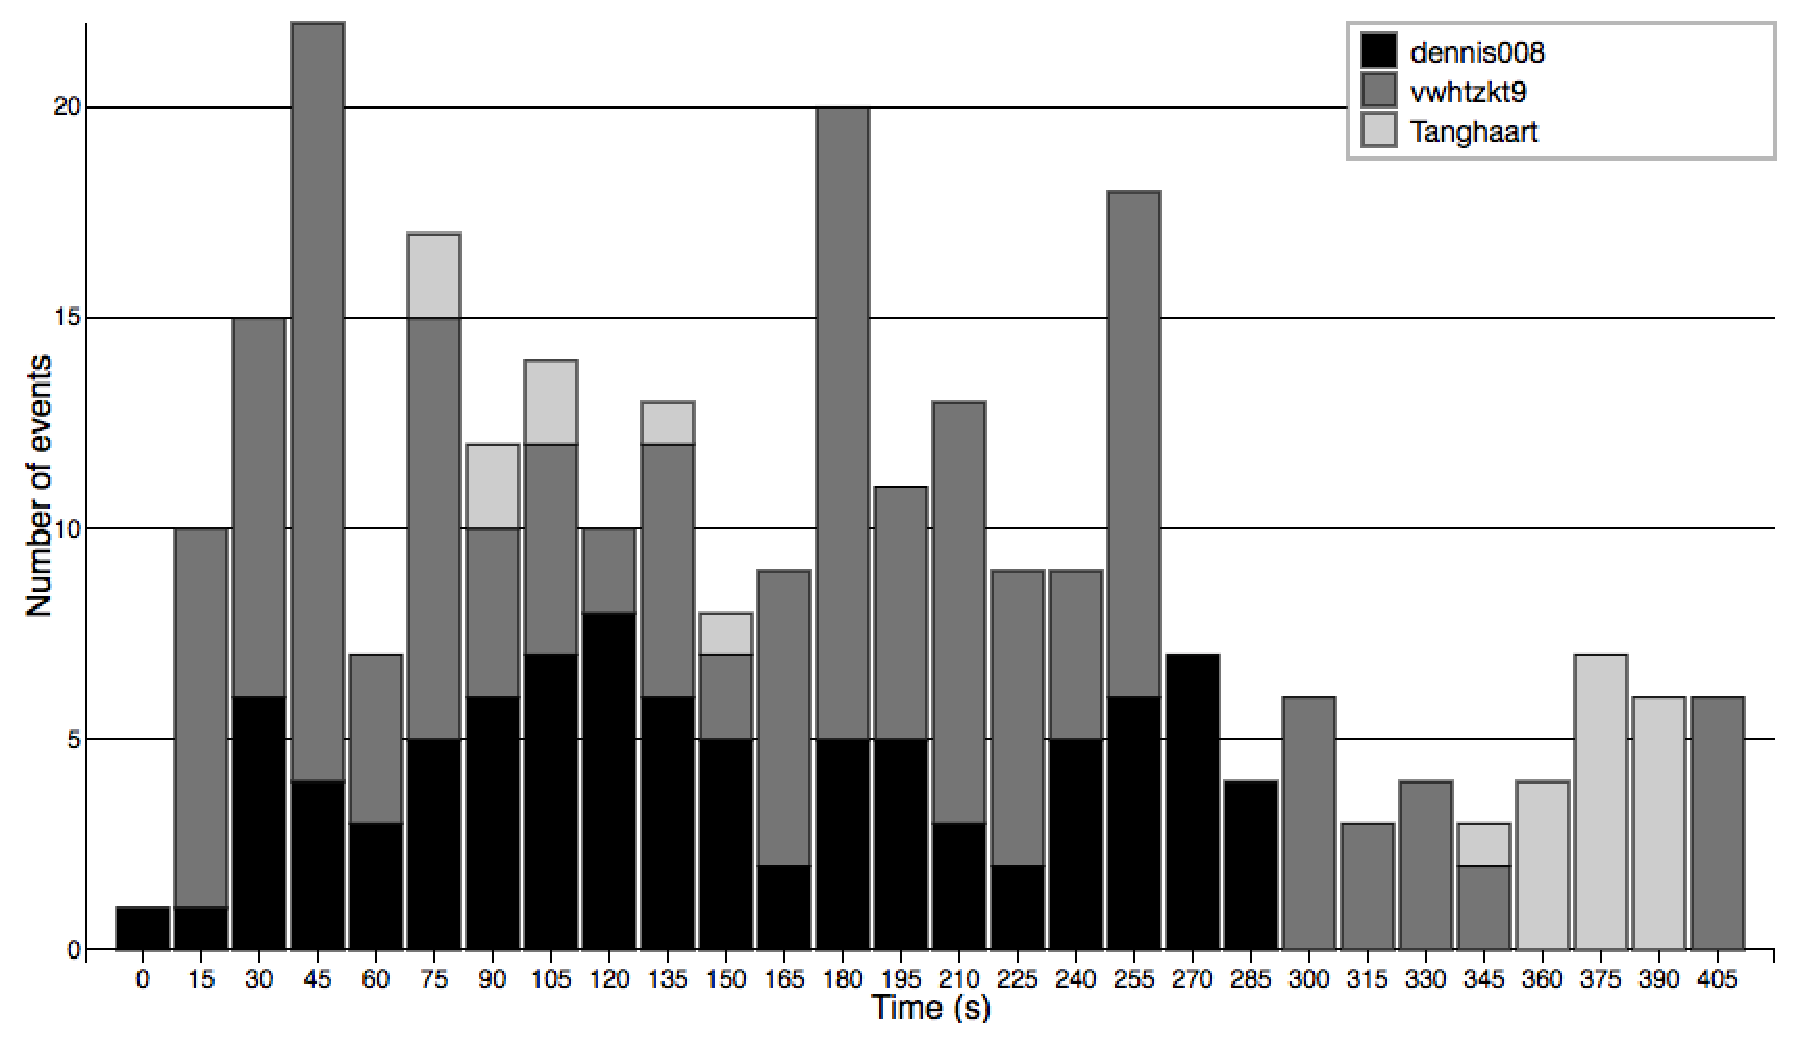
\includegraphics[width=0.8\textheight]{eps/byuser.eps}

\end{frame}

\begin{frame}{Bilan de l'approche orientée événements}
\begin{table}
	\begin{tabular}{lcc}
	\hline
	\textbf{QR}              & \multicolumn{2}{c}{\textbf{Approche orientée 
	événements}}  \\ 
	\hline
	\textbf{QR1 Réseau}      & \tick                             & Maillage partiel, flexibilité 
	(instances serveur)      \\
	\textbf{QR2 Traçabilité}  &          \tick                        & DDD et Event 
	Sourcing             \\
	\textbf{QR3 Autonomie}   & \tick                       & Stockage local 
	(haute dispo : donnnées, métier)      \\
	\textbf{QR4 Validité}    &     \tick                           &   DDD et CQRS               
	\\
	\textbf{QR5 Métriques}   & \tick (quali.)   \tickpartial 
	(quant.)                        &  Cohérence, Fiabilité, Robustesse, 
	Utilisabilité                           
	\\ 
	\hline
\end{tabular}
\end{table}
	\begin{description}

	\item[QR 2] La traçabilité est fournie par l'ES associée à la méthode DDD : 
	langage partagé de la 3D. ES fournit des données immuables et  
	fonctionnellement viables.
	
	\item[QR 3] L'utilisateur est rendu autonome par le fait de déporter CQRS et 
	ES 
	sur le client (traditionnellement client-serveur)
	
	\item[QR 4] Règles métiers fournies en amont par le DDD, validées par la 
	partie commande de CQRS
	
	%Comment les 
	%utilisateurs recoivent la chose....
\end{description}
\end{frame}

\begin{frame}{Testabilité de l'environnement virtuel collaboratif}
\begin{description}
	
	\item[QR 5] Quelles sont les critères permettant 
	d'évaluer un tel système de manière quantitative ? Qualitative ? 
	%Comment les 
	%utilisateurs recoivent la chose....
	
\end{description}
%Design and test DVEs
%\cite{Valadares2016}

%An architecture for client virtualization: A case study
Virtualisation complexe : WebRTC est une technologie récente \cite{Haque2016}


Nécessite l'intégration du modèle événementiel dans un logiciel de simulation.

De nombreuses variables : nombre de n\oe uds, types de scénarios, bande 
passante, taille des modèles 3D.

\begin{description}
	\item[temps de dissémination] d'un événement à travers le réseau
	\item[réactivité] face à la charge (nombre d'événements traités / seconde)
\end{description}



\end{frame}